%%% SETUP %%%%%%%%%%%%%%%%%%%%%%%%%%%%%%%%%%%%%%%%%%%%%%%%%%%%%%%%%%%%%%%%%%%%%%

%%% DOCUMENT TYPE %%%%%%%%%%%%%%%%%%%%%%%%%%%%%%%%%%%%%%%%%%%%%%%%%%%%%%%%%%%%%%

\documentclass[10pt,twocolumn, a4paper]{article}

%%% PACKAGES %%%%%%%%%%%%%%%%%%%%%%%%%%%%%%%%%%%%%%%%%%%%%%%%%%%%%%%%%%%%%%%%%%%

% Encoding

\usepackage[utf8]{inputenc}
\usepackage[T1]{fontenc}

% Geometry
\usepackage{multirow}
\usepackage{graphicx}
\usepackage{geometry} % edit margins of paper
\usepackage{setspace} % edit line spacing
\usepackage{fancyhdr} % header, footer
\usepackage{titlesec} % edit format of titles

% Visual

\usepackage[dvipsnames]{xcolor} % colors
\usepackage{tikz} % graphics
\usepackage[framemethod=tikz]{mdframed} % frames, better theorems

% Math

\usepackage{amsmath} % math tools
\usepackage{amssymb} % math symbols
\usepackage{amsthm} % thereoms
\usepackage{mathtools} % math tools

% Referencing

\usepackage{nameref}
\usepackage{hyperref}
\usepackage{cleveref}
% Useful

\usepackage[shortlabels]{enumitem} % enumerations

% Other

\usepackage{lastpage} % get number of last page

%%% MARGINS %%%%%%%%%%%%%%%%%%%%%%%%%%%%%%%%%%%%%%%%%%%%%%%%%%%%%%%%%%%%%%%%%%%%

\geometry{a4paper, left=20mm, right=20mm, top=20mm, bottom=20mm, includehead}

%%% COLORS %%%%%%%%%%%%%%%%%%%%%%%%%%%%%%%%%%%%%%%%%%%%%%%%%%%%%%%%%%%%%%%%%%%%%

%%% TITLES %%%%%%%%%%%%%%%%%%%%%%%%%%%%%%%%%%%%%%%%%%%%%%%%%%%%%%%%%%%%%%%%%%%%%

\colorlet{color-section}                {BrickRed}
\colorlet{color-subsection}             {BrickRed}

%%% MATH BOXES %%%%%%%%%%%%%%%%%%%%%%%%%%%%%%%%%%%%%%%%%%%%%%%%%%%%%%%%%%%%%%%%%

\colorlet{color-definition}             {SpringGreen!20}
\colorlet{color-theorem}                {Apricot!13}
\colorlet{color-proposition}            {Apricot!13}
\colorlet{color-corollary}              {Apricot!13}
\colorlet{color-lemma}                  {Apricot!13}
\colorlet{color-remark}                 {Gray!5}
\colorlet{color-example}                {Lavender!7}
% \colorlet{color-proof}                  {FILL COLOR HERE}


%%% CAPTIONS %%%%%%%%%%%%%%%%%%%%%%%%%%%%%%%%%%%%%%%%%%%%%%%%%%%%%%%%%%%%%%%%%%%

%%% CAPTION DEFINITION %%%%%%%%%%%%%%%%%%%%%%%%%%%%%%%%%%%%%%%%%%%%%%%%%%%%%%%%%

\newcommand*{\definitionname}{Definition}
\newcommand*{\theoremname}{Theorem}
\newcommand*{\propositionname}{Proposition}
\newcommand*{\corollaryname}{Corollary}
\newcommand*{\lemmaname}{Lemma}
\newcommand*{\remarkname}{Remark}
\newcommand*{\examplename}{Example}


%%% SHORTCUTS %%%%%%%%%%%%%%%%%%%%%%%%%%%%%%%%%%%%%%%%%%%%%%%%%%%%%%%%%%%%%%%%%%

%%% SINGLE SYMBOLS %%%%%%%%%%%%%%%%%%%%%%%%%%%%%%%%%%%%%%%%%%%%%%%%%%%%%%%%%%%%

% Logic

% \forall exists
% \exists exists
% \lnot exists
% \lor exists
% \land exists
\newcommand*{\limp}{\rightarrow}
\newcommand*{\limps}{\; \limp \;} % \limp with some space around
\newcommand*{\leqv}{\leftrightarrow}
\newcommand*{\leqvs}{\; \leqvs \;} % \leqv with some space around

% Meta Logic

% \implies exists
% \iff exists

% Colon Stuff

\newcommand*{\cl}{\colon}
\newcommand*{\cleq}{\coloneqq}
\newcommand*{\eqcl}{\eqqcolon}

% Sets

\newcommand*{\N}{\mathbb{N}} % natural numbers
\newcommand*{\Z}{\mathbb{Z}} % integers
\newcommand*{\Q}{\mathbb{Q}} % rational numbers
\newcommand*{\R}{\mathbb{R}} % real numbers
\newcommand*{\C}{\mathbb{C}} % complex numbers

%%% MATH OPERATORS %%%%%%%%%%%%%%%%%%%%%%%%%%%%%%%%%%%%%%%%%%%%%%%%%%%%%%%%%%%%%

% General

\DeclareMathOperator{\id}{id}
\DeclareMathOperator{\sgn}{sgn}

%%% TEMPLATES %%%%%%%%%%%%%%%%%%%%%%%%%%%%%%%%%%%%%%%%%%%%%%%%%%%%%%%%%%%%%%%%%%

% General

% write a set definition like: { #1 | #2 }
\newcommand*{\setdefinition}[2]{
  \left\{ #1 \mathrel{}\middle|\mathrel{} #2 \right\}
}

% write a nice map definition
\newcommand*{\mapdefinition}[5]{
  \begin{align*}
    #1 \cl #2 &\to     #3 \\
           #4 &\mapsto #5
  \end{align*}
}


%%% FORMATTING %%%%%%%%%%%%%%%%%%%%%%%%%%%%%%%%%%%%%%%%%%%%%%%%%%%%%%%%%%%%%%%%%

%%% HEADER, FOOTER %%%%%%%%%%%%%%%%%%%%%%%%%%%%%%%%%%%%%%%%%%%%%%%%%%%%%%%%%%%%%

\pagestyle{fancy}
\fancyhf{} % clear everything
\lhead{\sffamily}
\chead{\sffamily \large \bfseries Tichu strategies depending on course of play}
\rhead{\sffamily Page \thepage /\pageref*{LastPage}}
\lfoot{}
\cfoot{}
\rfoot{}

%%% TITLE FORMAT %%%%%%%%%%%%%%%%%%%%%%%%%%%%%%%%%%%%%%%%%%%%%%%%%%%%%%%%%%%%%%%

\setcounter{secnumdepth}{2}

\titleformat{\chapter}[display]
{\normalfont\huge\bfseries}{\chaptertitlename\ \thechapter}{20pt}{\Huge}
\titleformat{\section}[frame]
{\normalfont\LARGE\bfseries\color{color-section}\scshape}{\filright\,\thesection\,}{0.2ex}{\filcenter}
\titleformat{\subsection}
{\normalfont\Large\bfseries\color{color-subsection}}{\thesubsection}{1em}{}
\titleformat{\subsubsection}
{\normalfont\normalsize\bfseries}{\thesubsubsection}{1em}{}
\titleformat{\paragraph}[runin]
{\normalfont\normalsize\bfseries}{\theparagraph}{1em}{}
\titleformat{\subparagraph}[runin]
{\normalfont\normalsize\bfseries}{\thesubparagraph}{1em}{}

%%% SPACING %%%%%%%%%%%%%%%%%%%%%%%%%%%%%%%%%%%%%%%%%%%%%%%%%%%%%%%%%%%%%%

% Titles

\titlespacing*{\chapter}{0pt}{50pt}{40pt}
\titlespacing*{\section}{0pt}{3.5ex plus 1ex minus .2ex}{2.3ex plus .2ex}
\titlespacing*{\subsection}{0pt}{3.25ex plus 1ex minus .2ex}{1.5ex plus .2ex}
\titlespacing*{\subsubsection}{0pt}{3.25ex plus 1ex minus .2ex}{1.5ex plus .2ex}
\titlespacing*{\paragraph}{0pt}{3.25ex plus 1ex minus .2ex}{1em}
\titlespacing*{\subparagraph}{\parindent}{3.25ex plus 1ex minus .2ex}{1em}

% Text, Paragraphs

%\setstretch{1.05} % scaling of space between lines
\setlength{\parindent}{0pt} % indentation of paragraphs
%\setlength{\parskip}{4.0pt plus 1.0pt minus 1.0pt} % space between paragraphs
\setlength{\parskip}{0.8ex}
\setlength{\topsep}{0pt}

%%% SYMBOLS USED BY NUMBERINGS, ENVIRONMENTS, ... %%%%%%%%%%%%%%%%%%%%%%%%%%%%%%

% \renewcommand*\qedsymbol{$\blacksquare$} % alternative QED symbol
\renewcommand{\thefootnote}{\arabic{footnote}} % normal footnotes on page
\renewcommand{\thempfootnote}{\fnsymbol{mpfootnote}} % footnotes on minipages, e.g. in mdframed environments

%%% LISTS, ENUMERATIONS %%%%%%%%%%%%%%%%%%%%%%%%%%%%%%%%%%%%%%%%%%%%%%%%%%%%%%%%

% 'itemize'

\setlist[itemize]{noitemsep, topsep=0pt}

% 'enumerate'

% no special settings at the moment

% 'description'

% no special settings at the moment

% 'axioms'

\newlist{axioms}{enumerate}{2}
\setlist[axioms]{itemsep=0pt,label*=\arabic*.}

%%% MDFRAMED PATCH %%%%%%%%%%%%%%%%%%%%%%%%%%%%%%%%%%%%%%%%%%%%%%%%%%%%%%%%%%%%%

\usepackage{xpatch}

\makeatletter
\xpatchcmd{\endmdframed}
  {\aftergroup\endmdf@trivlist\color@endgroup}
  {\endmdf@trivlist\color@endgroup\@doendpe}
  {}{}
\makeatother

%%% MDFRAMED STYLES %%%%%%%%%%%%%%%%%%%%%%%%%%%%%%%%%%%%%%%%%%%%%%%%%%%%%%%%%%%%

% thick frame and bar for title

\mdfdefinestyle{style-box}{
  skipabove=1.5ex plus .5ex minus .2ex,
  skipbelow=1ex plus .2ex minus .2ex,
  linewidth=2pt,
  linecolor=Gray!20,
%   roundcorner=3pt,
  innerleftmargin=0.5\baselineskip,
  innerrightmargin=0.5\baselineskip,
  innertopmargin=0.4\baselineskip,
  innerbottommargin=0.4\baselineskip,
  frametitlebackgroundcolor=Gray!20,
  frametitleaboveskip=0.3pt,
  frametitlebelowskip=0.3pt,
  theoremseparator=,
  theoremspace=\hfill,
  theoremtitlefont=\mdseries\scshape,
  nobreak=true
}

% highlighted background

\mdfdefinestyle{style-background}{
  skipabove=1.5ex plus .5ex minus .2ex,
  skipbelow=1ex plus .2ex minus .2ex,
  hidealllines=true,
  backgroundcolor=Gray!5,
  innerleftmargin=0.5\baselineskip,
  innerrightmargin=0.5\baselineskip,
  innertopmargin=0.4\baselineskip,
  innerbottommargin=0.4\baselineskip,
}

% thin frame

\mdfdefinestyle{style-leftline}{
  skipabove=1.5ex plus .5ex minus .2ex,
  skipbelow=1ex plus .2ex minus .2ex,
  linewidth=1pt,
  linecolor=Gray!50,
  topline=false,
  bottomline=false,
  rightline=false,
  innerleftmargin=0.5\baselineskip,
  innerrightmargin=0,
  innertopmargin=0.2\baselineskip,
  innerbottommargin=0.0\baselineskip,
}

%%% ENVIRONMENTS %%%%%%%%%%%%%%%%%%%%%%%%%%%%%%%%%%%%%%%%%%%%%%%%%%%%%%%%%%%%%%%

% Definition

\mdtheorem[
  style=style-box,
  linecolor=color-definition,
  frametitlebackgroundcolor=color-definition
]{definition}{\definitionname}[section]

% Theorem

\mdtheorem[
  style=style-box,
  linecolor=color-theorem,
  frametitlebackgroundcolor=color-theorem,
  font=\itshape
]{theorem}{\theoremname}[section]

% Proposition

\mdtheorem[
  style=style-box,
  linecolor=color-proposition,
  frametitlebackgroundcolor=color-proposition,
  font=\itshape
]{proposition}[theorem]{\propositionname}

% Corollary

\mdtheorem[
  style=style-box,
  linecolor=color-corollary,
  frametitlebackgroundcolor=color-corollary,
  font=\itshape
]{corollary}[theorem]{\corollaryname}

% Lemma

\mdtheorem[
  style=style-box,
  linecolor=color-lemma,
  frametitlebackgroundcolor=color-lemma,
  font=\itshape
]{lemma}[theorem]{\lemmaname}

\theoremstyle{remark}

% Remark

\newtheorem*{remark}{\remarkname}
\surroundwithmdframed[
  style=style-background,
  backgroundcolor=color-remark
]{remark}

% Example

\newtheorem*{example}{\examplename}
\surroundwithmdframed[
  style=style-background,
  backgroundcolor=color-example
]{example}

% Proof

\surroundwithmdframed[
  style=style-leftline
]{proof}

%%% TEXT FORMATTING %%%%%%%%%%%%%%%%%%%%%%%%%%%%%%%%%%%%%%%%%%%%%%%%%%%%%%%%%%%%

% definitions

\newcommand*{\df}[1]{\textbf{#1}}



%%% LANGUAGE %%%%%%%%%%%%%%%%%%%%%%%%%%%%%%%%%%%%%%%%%%%%%%%%%%%%%%%%%%%%%%%%%%%

%%% SETUP %%%%%%%%%%%%%%%%%%%%%%%%%%%%%%%%%%%%%%%%%%%%%%%%%%%%%%%%%%%%%%%%%%%%%%

\usepackage[english]{babel}

%%% CAPTION REDEFINITION %%%%%%%%%%%%%%%%%%%%%%%%%%%%%%%%%%%%%%%%%%%%%%%%%%%%%%%



%%% HYPHENATION %%%%%%%%%%%%%%%%%%%%%%%%%%%%%%%%%%%%%%%%%%%%%%%%%%%%%%%%%%%%%%%%




%%% DOCUMENT %%%%%%%%%%%%%%%%%%%%%%%%%%%%%%%%%%%%%%%%%%%%%%%%%%%%%%%%%%%%%%%%%%%
%\usepackage{slashbox}
\usepackage{multirow}
\usepackage{listings}

\begin{document}

\title{Tichu strategies depending on course of play}
\date{June 03, 2020}
\author{Matthias Schmickler \and Paul Sander \and Jean-Luc Portner \and Tom Haidinger \and Andrey Bryutkin \\ \\ Swiss Federal Institute of Technology Zurich (ETH)}
\maketitle

\section{Motivation and goals}

A prevalent characteristic of both mathematics and physics is their elaborate structure of interdependent concepts. It is only natural, then, for us students to thrive off of complexity and intricateness both within our courses as well as throughout our daily life. One such endeavour we satisfy our free time with is the game of Tichu. Tichu is a team card game taught to us by older students of our courses during the, albeit not very wide-ranging, cultural melting-pot between years – that unproductive period when our courses’ study hall slowly turns into the Mensa. 

    In addition to luck and strategy, this game became popular within our friend-group due to its fairly unique aspect of interaction. Allowing for multiple possible card combinations, special cards and a process of card switching, Tichu derives its complexity not through complicated rules, but rather through diverseness of strategy. Indeed, given one must adapt to one’s opponents’ and teammate’s strategies, one may say its strategies are interactive and reactive in nature. Therefore – although we note that card games are hard to analyse in general – we believe Tichu is indeed approachable through game-theoretic methods. 

    Fascinated by this type of game and equipped with tools from our game theory course, we pose the general question: “which strategy should we pursue as players?”. We shall further differentiate this admittedly vague question into: “what strategy should we pursue given”: a) “we know what player-type all other players are” and b) “we do not know anything about other players”. 
\section{Introduction on Tichu}

Tichu is played by four players, where two players form a team. Tichu is subdivided into subgames, which are played repeatedly until one team reaches 1000 points and in this way wins the game.
At the beginning of a game, every player gets 14 cards. He exchanges one card with every other player. This will be called the "Exchange Stage", which we will discuss later on. After the exchange of the cards, the regular game takes place. There are two major ways to achieve points: 1st Claiming Cards with a value, 2nd Announcing a Tichu. The Game ends, when one team finished of their cards. If one team finished of their cards before one of the opposing team finished, then the winner team receives the cards from both opponent players. If the team finished of their cards and someone from the opposing team finished before, only the last player passes away the cards to the winner team. Then you count the values of the cards and this value to your score.

A Tichu-set consists of the cards 2, 3, 4, 5, 6, 7, 8, 9, 10, J, Q, K, A in four different colors: red, blue, green and black. There are four special cards Dragon, Phoenix, Dogs and Mah Jong. In total we have 56 cards, every player receives 14 cards. However, only a few cards have a value as listed in the table:\\
\begin{scriptsize}
\begin{center}
\begin{tabular}{ c c c }
\textbf{5} & $\sim$  & \textbf{5 P} \\
\textbf{10} & $\sim$ & \textbf{10 P} \\
\textbf{K} & $\sim$  & \textbf{10 P} \\
\textbf{Dragon} & $\sim$ & \textbf{25 P} \\
\textbf{Phoenix} & $\sim$ & \textbf{-25 P}
\end{tabular}
\end{center}
\end{scriptsize}
In total, there are 100 Points every round. It is also possible to win a game with 125 or also -25 Points. Announcing a Tichu can earn your team additional points.
A game starts, when a player plays a valid combination. The other players can now try to play a higher version of the same combination (as many cards as the combination). If no player can or wants to play a higher combination, the player with the highest combination takes the cards and can play a new combination. There are several valid combinations:
\\
\\
\resizebox{0.5\textwidth}{!}{%
\begin{tabular}{ c c c }
\textbf{High Card} & $\sim$  & \textbf{2 $<$ 3 $< ... <$ A} \\
\textbf{Pair} & $\sim$ & \textbf{(2,2) $< ... <$ (A,A)} \\
\textbf{Triple} & $\sim$  & \textbf{(2,2,2) $< ... <$ (A,A,A)} \\
\textbf{Following Pairs} & $\sim$ &  \textbf{(2,2,3,3, ...) $< ... < $ (..., K,K,A,A)}
 \\
\textbf{Full House} & $\sim$ &  \textbf{(2,2,2,A,A) $<... <$ (A,A,A,K,K)} \\
\textbf{Street(more than 5 cards)} & $\sim$ & \textbf{(2,3,4,5,6, ...) $< ... < $(...,10,J,Q,K,A)}
\end{tabular}%
}

This combinations can only be played on the same combination when it is the players turn. Following Pairs and Streets can be continued up to 14 cards. There are also bombs, which can be played at any time and on every combination (except higher or equal bombs).
We differ between two kinds of bombs:
\\
\\
\resizebox{0.5\textwidth}{!}{%
\begin{tabular}{ c c c }
\textbf{Bomb} & $\sim$  & \textbf{(2,2,2,2), $< ... <$ (A,A,A,A)} \\
\textbf{Street Bomb} & $\sim$ & \textbf{(A,A,A,A) $<$ (2,3,4,5,6) $<$ (2,3,4,5,6, ...) $< ... < $ (...,10,J,Q,K,A)} \\ \\
\end{tabular}%
}
In a street Bomb all colors have the same color. A Street Bomb is always higher than a shorter Street Bomb or a regular Bomb.

The four special cards can be played under certain conditions,but special cars can not be player in a Bomb or Streetbomb:

\paragraph*{Mah Jong}
The player with this card starts the game. Mah Jong can be played as a \textbf{1} as a High Card or in a Street. The player is also allowed to request a not special card. Whoever has this card and can play it, has to play it.
\paragraph*{Dog}
The dogs can not be played in any combination. When a player uses the dog, his partner is allowed to play the next combination. If his partner is already done, the next active player is allowed to play.
\paragraph*{Phoenix}
The phoenix can be used in two different ways. It is a valid substitute for every not special card and can be played in combinations. It can also be played on a card and count as Card + 0.5. It can also be used on an A but not on the Dragon.
\paragraph{Dragon}
The dragon is the highest High Card and can be played on every high card including the phoenix. After winning the combination with the dragon, the player has to give the cards to qqone of his enemies.

\subsubsection{Announcing a Tichu}
A Player can announce a Tichu as long as he has not played any card yet. If he announces a Tichu, he has to be the first one who finishes the game. If he succeeds, he will earn his team 100 additional points. If he fails, his team loses 100 points. 
A stronger version of Tichu is the Great Tichu, which is worth 200 points if won. A Great Tichu has to be announced after the player takes the first eight cards before the regular game starts. It also has an impact on the Exchange Stage. 
If the two players from one team finish the game first, they get 200 points and the cards will not be counted. This will be called a “Double Victory”.

\section{Our Model and approximations}
\subsection{Basic assumptions}
Our basic approximation consists of two distinctions regarding player behavior and transparency of information. 

In our consideration we would like to define the following two types of players.
The first player is the "aggressive player" - he is characterized by the fact that he takes a higher risk and pays more attention to the value of his cards and less to his playing partner. In case of doubt he will keep the good cards and give his partner something worse than the other way round.
The willingness to take risks is characterized by the fact that even with below average cards (relative to cards with which the average player would announce a tichu) he already announces the tichu. 

The second player is the "defensive player". This stands in contrast to the "aggressive player type". He is rather risk-averse, which means he needs above average (relative to cards with which the average player would announce a tichu) good cards to announce a tichu.
When exchanging cards he decides to give the good card to his partner instead of keeping it himself.

To make it easier to identify the players in the following, the following notation is introduced:
We will store information on the players behaviour in a vector $\alpha \in \{0,1\}^4$.
\\ 
\begin{itemize}
\item A: "aggressive player" will be assigned to $\alpha_i = 1$
\item D: "defensive player" will be assigned to $\alpha_i = 0$ \\
\end{itemize} 
In our approximation of Tichu, we consider two possible situations. 
The first situation is characterized by transparency. Every player knows exactly which type the other players are and acts up to this information.
In the second situation, the players are not aware of the tactics. They only know how they act by themself.

Like the different types of players, we will identify the situations with the following notation. The information is stored in a vector $\beta \in \{0,1\}^4$. \\ 
\begin{itemize}
\item T: “transparent” will be assigned to $\beta_i = 1$
\item $\overline{T}$: “not transparent” will be assigned to $\beta_i = 0$ \\
\end{itemize}

We will assume  $\beta_i = \beta_j \forall i, j\in \{1,2,3,4\}$ in the beginning. 

We also introduce the possibility to take a higher risk depending on the current score. If a player is risky, he will definitely announce a Tichu. If he is shy, he will never announce a Tichu. We will store information on the player's possibility to announce a tichu in a vector $\gamma \in \{0,1\}^4$. \\
\begin{itemize}
\item R: “risky” will be assigned to $\gamma_i = 1$
\item $\overline{R}$: “not risky” will be assigned to $\gamma_i = 0$ \\
\end{itemize}
While $\alpha$ is invariant, $\gamma$ is dynamically changing throughout the game. 

Our last variables will be the actual score of each team and the rounds played, which will be stored in $\delta \in \mathbb{Z}^4$. 
$\delta_{1,2} \widehat{=}$ total score, $\delta_{3,4} \widehat{=}$ last round score

We have also adopted the following approximations about the game.
The Great Tichu, i.e. the announcement of a Tichu before the exchange of cards, is very rare and is therefore negligible for our basic model.
Also the possibility to announce a Tichu during the game, i.e. when other players have already played cards, is neglected.
Furthermore, all rules are known to the players ("common knowledge") and they act rational to win the game and not harm their own team. 

\subsection{Introducing the game model}

\begin{figure}[h]
    \centering
    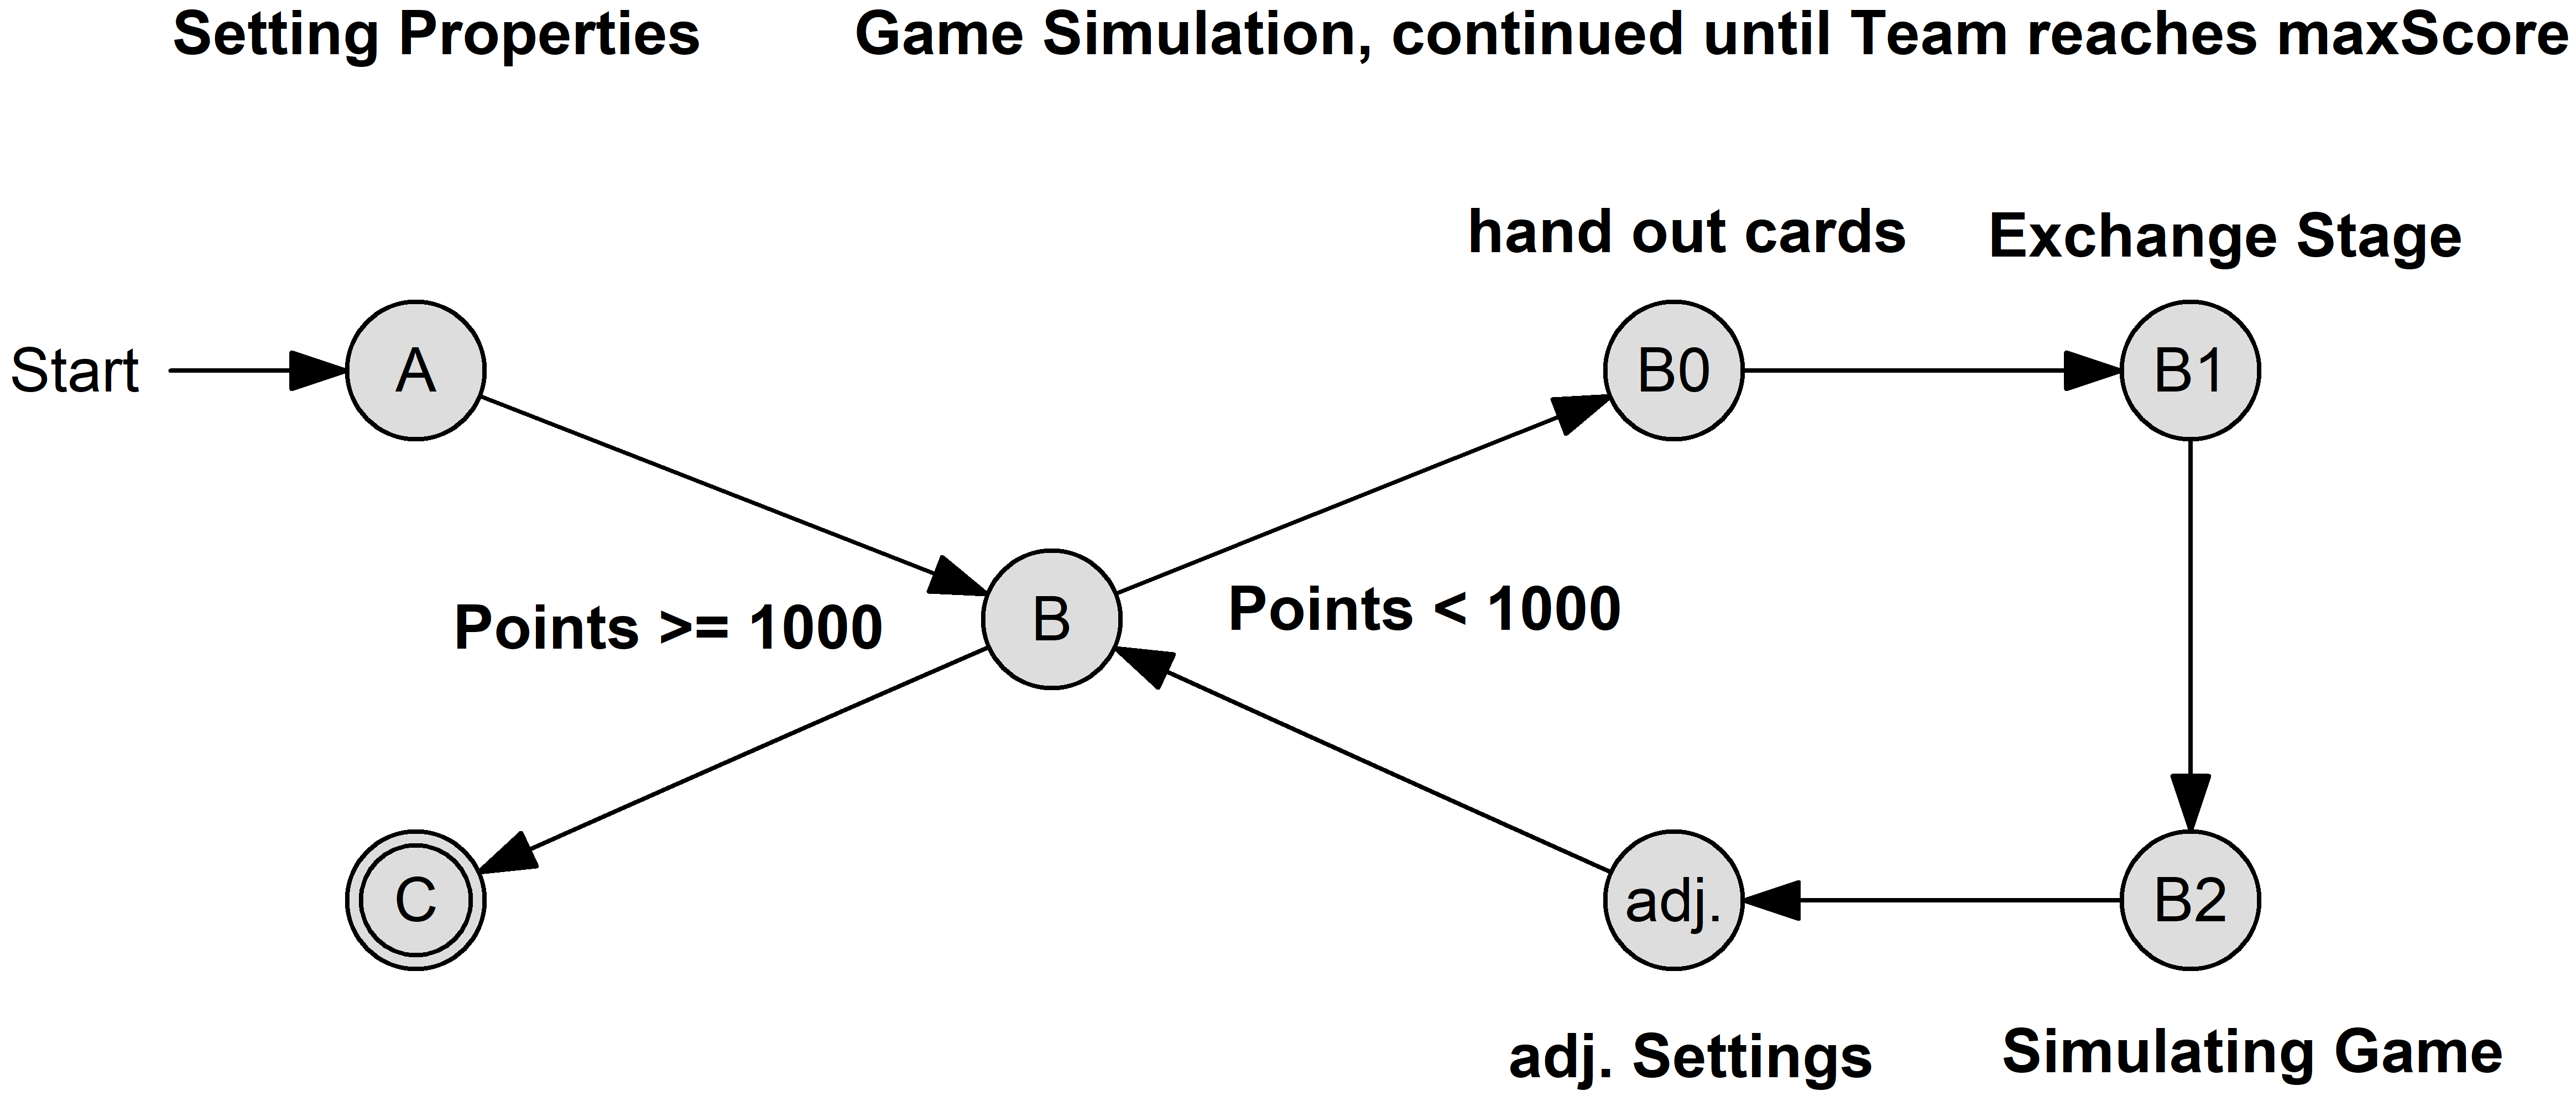
\includegraphics[width=0.5\textwidth]{Bilder/graph}
    \caption{Game model}
    \label{fig:meine-grafik}
\end{figure}

The game up to 1000 points is represented as a game tree.
At the beginning 4 players, divided into 2 teams enter the game (A). We will set $\alpha$ and $\beta$. 
The next part of the game (B) will be repeated until the score reaches at least 1000 points. We divided it into three subgames (B.0, B.1, B.2).
First, we will give every player a set of cards (B.0). This set of cards will be represented by a value $X_i$ in [0,1]. The sum of all sets can be higher than 1 in total. The value of the set is not connected to single cards but to a probability to play these cards in combinations. We will discuss this in detail later on.

In the basic model, B.0 is only connected to statistics and no game in meanings of game theory. Later on, we can introduce game-theoretical elements to this subgame. 

The second part (B.1) represents the “Exchange Stage”. Depending on his Cards and his strategy, every player will give away three $\Delta x$ and will receive three $\Delta x$ which can be positive or negative. The payoff will be represented by a Util$\in [0,1]$ with "new" card values.

The third subgame (B.2) takes the card values X from subgame B.1 and the score. They are used to determine the outcome of the actual game, reflecting on the players strategies and possibilities to take a higher risk because of the score. This will result in a Util function which allocates the 100 points (and additional Tichu-points) to the teams. 

To every game B, the parameters $\alpha, \beta, \gamma, \delta$ are considered and can be adjusted.  
The repetition of subgame B will end when one team reaches at least 1000 points. 

In first approximations we will also consider $\beta$ and $\gamma$ as invariant. 

\subsubsection{Subgame A}
To start a round of Tichu, we will assign a player $\alpha_i$ and $\beta_i$. As assumed before, all $\beta_i$ are equal. Therefore, we will have two options on $\beta$ and 16 options on $\alpha$. Some of those options are only permutations, because of the team-aspect. We will reduce the number of possible $\alpha$ to 6 as shown in the table. We will call this combination $\tilde{\alpha}_i$: \\
\begin{table}[h]
\resizebox{0.5\textwidth}{!}{%
\begin{tabular}{|c|c|c|}
\hline 
Player 1 $\backslash$ Player 2 & A & B \\ 
\hline 
A & 1 (AA) & 2 (AD = DA) \\ 
\hline 
B & 2 (DA = AD) & 3 (DD) \\
\hline 
\end{tabular}%
}
\end{table}
\begin{table}[h]
\resizebox{0.5\textwidth}{!}{%
\begin{tabular}{|c|l|l|l|}
\hline 
Player 1 $\backslash$ Player 2 & 1 & 2 & 3 \\ 
\hline 
1 & $\alpha_1$ (AAAA) & $\alpha_2$ (AAAD) & $\alpha_3$ (AADD) \\ 
\hline 
2 & $\alpha_2$ (ADAA) & $\alpha_4$ (ADAD) & $\alpha_5$ (DDAD) \\ 
\hline 
3 & $\alpha_3$ (DDAA) & $\alpha_5$ (ADDD) & $\alpha_6$ (DDDD) \\ 
\hline 
\end{tabular}%
} 
\end{table}
\subsection{Subgame B.0}
In our basic model, B.0 is invariant under all $\alpha$, $\beta$, $\gamma$ and $\delta$. It is only based on statistics. 
To start off with a simple approximation, we assign $X_i$ to be an element of the normal distribution with parameters $\mu$, $\sigma$.
Our first assumptions is, that we set $\mu$ to 0.5 and will define $X_i$ higher or equal to 1 as 1,  $X_i$ lower or equal to 0 as 0.   
According to this definition, $X_i$ is always in $[0,1]$. We will set $\sigma$ later according to realistic data and surveys. We will now assume that we will always get an $X = \{X_1, …, X_4\}$ from subgame B.0. This will be the card value used in later games. 

\subsection{Subgame B.1}
To understand the “Exchange Stage”, we have to give some basic information on Tichu which leads to our approximation of this subgame. First of all we definie some terms:
\begin{definition}["good" cards]
"Good" cards are for example bombs, high cards like ace or long, specific combinations that other players do not have.
\end{definition}
\begin{definition}["bad" cards]
Bad cards can rarely be played, for example deep cards or combinations that are never the highest combinations, so you rarely win a trick
\end{definition}
\begin{enumerate}
\item A player can give “good” cards to his partner if and only if he has “good” cards.
\item A player can give “bad” cards to his opponents if and only if he has “bad” cards. 
\item The value of a card is subjective to a player. 
\item There is no absolute solution for every situation, the best solution is subjective to a player \\
\end{enumerate}
\begin{definition}[Player, Team, Partner and Opponent]
Given $\alpha$, $\beta$ and $X$, a player $P_i$ is called the triple ($\alpha_i$, $\beta_i$, $X_i$). 
On the set of players, we define an equivalence relation, where each class forms a Team $T_j$. Following conditions are true for players A ($\alpha_A$, $\beta_A$, $X_A$), B($\alpha_B$, $\beta_B$, $X_B$), C($\alpha_C$, $\beta_C$, $X_C$):
 \begin{axioms}[(P1)]
  \item A $\sim $ B (Reflexiv)
  \item A $\sim$ B $\Leftrightarrow$ B $\sim$ A (Symmetric)
  \item A $\sim$ B, B $\sim$ C $\Rightarrow$ A $\sim$ C (Transitivity)
  \end{axioms}
Players in the same Team will be called partners while players in another Team will be called opponents. We will write $PT_i$ for the Partner Team of $P_i$ and $OT_i$  for the Opponent Team of $P_i$.

We define $T_1 = [P_1,P_2]$  and $T_2 = [P_3,P_4]$. Therefore, $PT_1 = T_1$, $OT_1 = T_2$, $PT_2 = T_2$, $OT_2 = T_1$.

\end{definition}

\begin{definition}[Symmetric game perspective]
We will say, two players $P_i$, $P_j$ with  $i \neq j$ share a symmetric game perspective if $P_i = P_j$, $PT_i = PT_j$, $OT_i = OT_j$, in words: They have the same cards and the teams are identically from their point of view. 
\end{definition}
\begin{definition}[Total Exchange-Function]
We assume we have given $\alpha$, $\beta$, X. A function $\pi: \{0,1\}^8 \times [0,1]^4 \to [0,1]^4, (\alpha, \beta, X) \mapsto (X’)$ will be called an Exchange-function to B.1  if it applies to the following rules:
\paragraph{Randomness and Average}
$\alpha$, $\beta$, X are fixed. Then there is $\Delta X \subset [0,1]^4$ with $X’ \in \Delta X$. We will write $\pi^* (\alpha, \beta, X) = X^* \in \Delta X$ for the average of $\pi(\alpha, \beta, X)$. $\pi^*$ is a well-defined function, while $\pi$ allows random values around $\pi^*$.
\paragraph{Continuous and monotony of X}
$\alpha$, $\beta$ and X are fixed. If we change X in only one value that $X_i$ becomes $wide\hat{X_i}$, it applies to the following rules:
\begin{axioms}[(C1)]
\item $\forall \epsilon > 0, \exists \delta > 0$ with $| X_i - \widehat{X_i}| < \delta$ \\$\Rightarrow | \pi^*(X_i) - \pi^*(\widehat{X_i}) | < \epsilon $
\item $\widehat{X_i} \leq X_i \Rightarrow \pi^*(\widehat{X_i}) \leq \pi(X_i)$
\end{axioms}

\paragraph{Symmetric outcome}
If two players $P_i$, $P_j$ have a symmetric game perspective, $\pi^*(X_i) = \pi^*(X_j)$
\end{definition}

Based on our approximations of the subgame, we now try to construct an Exchange Function. First of all, we try to create an easier function, which describes how a single Player selects cards he wants to give away. If we only look at this function, we will see some facts:

\begin{axioms}[(F1)]
\item For Player $P_i$, only $\alpha$, $\beta_i$ and $X_i$ are relevant.
\item Player $P_i$ does not differ between Opponents. 
\item The Player $P_i’s$ strategy does not change his behaviour on Opponents. 
\item In fact, he only needs to know his strategy, who he selects cards for and if known, his partner’s strategy. 
\end{axioms}

We put these facts together in a Diagram (the numbers represent diffrent exchange functions and $P_P$ - is a Player passing; $P_R$ - is a Player receiving):

\begin{table}[h]
\caption{Table 1.1} \bigskip
\label{tab:my-table}
\resizebox{0.5\textwidth}{!}{%
\begin{tabular}{l|l|ll|l|ll|}
\cline{2-7}
                                          & \multicolumn{3}{l|}{$\beta_i = 0$} & \multicolumn{3}{l|}{$\beta_i=1$} \\ \hline
\multicolumn{1}{|l|}{\multirow{3}{*}{OT}} & $P_R \backslash P_P$           & A         & D         &           & A         & D        \\ \cline{2-7} 
\multicolumn{1}{|l|}{}                    & A          & 1         & 1         & A         & 2         & 2        \\
\multicolumn{1}{|l|}{}                    & D          & 1         & 1         & D         & 2         & 2        \\ \hline
\multicolumn{1}{|l|}{\multirow{3}{*}{PT}} & $P_R \backslash P_P$              & A         & D         &           & A         & D        \\ \cline{2-7} 
\multicolumn{1}{|l|}{}                    & A          & 3         & 4         & A         & 5         & 6        \\
\multicolumn{1}{|l|}{}                    & D          & 3         & 4         & D         & 7         & 8        \\ \hline
\end{tabular}%
}
\end{table}
\paragraph{1.}
The Player is exchanging with an unknown Opponent. Therefore he will select a “bad” card, independent of his own strategy
\paragraph{2.}
The Player knows his opponent. He will also give him a “bad” card. The only difference is, that he knows better how the player will react on the card. This will change how an Opponent receives the card, but is equivalent to 1. 
\paragraph{3./4.}
The Player gives cards to his Partner depending on his strategy. He does not know the strategy of his Partner.
\paragraph{5.-8.}
The Player knows his own and his Partners strategy. Therefore his results will be better and the card difference will change. 

\begin{definition}[Pass-Function]
A function $\xi_{ji} : \{0,1\}^5 \to [-1,1], (\alpha, \beta_i) \to \hat{\xi}_{ji}$ will be called a pass function, if it describes what $P_i$ gives to $P_j$ according to certain rules:
\paragraph{Randomness and Average}
$\alpha$, $\beta_i$ are fixed. Then there is $\Delta  \hat{\xi_{ji}} \subset [-1,1]$ with  $\hat{\xi_{ji}} \in \Delta  \hat{\xi_{ji}}$. We will write $\{xi_{ji}\}^* (\alpha, \beta_i) =  \hat{\xi_{ji}} \in \Delta  \hat{\xi_{ji}}$ for the average of $\xi(\alpha, \beta_i)$. $\xi_{ji}^*$ is a well-defined function, while $\xi$ allows random values around $\xi^*$.
\paragraph{Symmetric outcome}
If two players $P_i$, $P_j$ have a symmetric game perspective towards each other,  $\hat{\xi_{ji}}^* =  \hat{\xi_{ji}}^*$
\paragraph{Normative aspects}
$\sum_{j = 1}^4 \hat{\xi_{ji}} = 1$
\paragraph{Realistic passing}
$\hat{\xi_{ii}} >>  \hat{\xi_{ji}}$ with $ i \neq j $
\end{definition}
\begin{definition}[Receive-Function]
A function $\eta_{ji}: \{0,1\} \times [-1,1] \to [-1,1], (\beta_i,  \hat{\xi_{ji}}) \mapsto \hat{\eta_{ji}}$ will be
called a “Receive-Function”, if it describes how $P_j$ receives cards from $P_i$ according to certain rules:
\paragraph{Randomness and Average}
$\beta_i$, $\hat{\xi_{ji}}$ are fixed. Then there is $\Delta  \hat{\eta_{ji}} \subset [-1,1]$ with  $\hat{\eta_{ji}} \in \Delta  \hat{\eta_{ji}}$. We will write $\{\eta_{ji}\}^* (\beta_i, \hat{\xi_{ji}}) =  \hat{\eta_{ji}} \in \Delta  \hat{\eta_{ji}}$ for the average of $\eta(\beta_i, \hat{\xi_{ji}})$. $\eta_{ji}^*$ is a well-defined function, while $\eta$ allows random values around $\eta^*$.
\paragraph{Symmetric outcome}
If two players $P_i$, $P_j$ have a symmetric game perspective towards each other:  $\hat{\xi_{ji}}^* =  \hat{\xi_{ij}}^*$
\paragraph{Self passing}
$\eta_{ii}(\hat{\xi_{ii}}) = \hat{\xi_{ii}} $
\end{definition}
\begin{definition}[Exchange-Function]
A function $\lambda_{ji}: \{0,1\}^5 \to [-1,1], \lambda_{ji} = \eta_{ji} \circ \xi_{ji}$ with $\eta_{ji}$ a Receive-Function and $\xi_{ji}$ a Pass-Function with existing $\alpha$, $\beta_i$.
\end{definition}
\begin{remark}[Construction]
We will now construct a Total Exchange Function based on an Exchange Function $\lambda_{ji}$. We will define $\Lambda = (\lambda_{ji})$ as a quadratic matrix. 
The Total Exchange-Function will be $\Lambda: X \mapsto \Lambda X = X’$
We now have to prove that this construction fits the definition.
\begin{axioms}[(1)]
\item Randomness and Average: This is induced from the combination of $\xi_{ji}$ and $\eta_{ji}$ in every argument. Therefore we can find an $\Delta \Lambda$ and $\Lambda^* $ which lead to $\Delta X $ and 
$X^*$
\item $\Lambda^*$ is a linear function, therefore continuous and monotone
\item Symmetric outcome is induced from the combination of $\xi_{ji}$ and $\eta_{ji}$ in every argument as in 1
\end{axioms}
We have now created a matrix $\Lambda$ which describes the Exchange Stage. To complete the definitions, we will introduce $ \Pi : \{0,1\}^8 \to M(4 \times 4, \mathbb{R}), (\alpha, \beta) \mapsto \Lambda $
\end{remark}

\subsection{Subgame B.2}
In this subgame we look at the playing of the active game, i.e. the laying of cards and the trimming of other cards. Again, we assume that these are rational players who do not harm their own team. This means that if one player of a team has announced a tichu, the other player would not announce a counter tichu. Therefore we can make the assumption that we consider each team as one element playing together against the other.
As a reminder, teams are defined by combining the two player triples $P_1$, $P_2$ and $P_3$, $P_4$into one element $T_1 = \{P1,P2\}$ and $T_2 = \{P3,P4\}$.

Let S be the score of the game given by $S = \{S_1, S_2\} \in \mathbb(Z)^2$ where $S_1$ and $S_2$ are the score of each team.
\begin{definition}[Tichu Announcement Probability]
Now we define a function $C_i(T_i, S)$ for each team, where $T_i$ is the respective team and S is the current score:
\begin{align*}
C_i: \{0,1\}^5 \times [0,1]^2 \times \mathbb{Z}^2 &\to [0,1] \\ (T_i,S) &\mapsto c_i
\end{align*}
\end{definition}
 These functions return the Tichu announcement probability of each team in this round. This clearly depends on the playing strategy of the players or the team as well as on the current score and the difference in points. E.g. this probability could increase if the difference in points becomes bigger or if the opponent team is much closer to 1000 than your own.

\begin{definition}[double win propability]
Furthermore, define a function $D_i(T_1, T_2)$ for each team:
\begin{align*}
D_i: \{0,1\}^5 \times [0,1]^4 &\to [0,1] \\ (T_1,T_2) &\mapsto d_i
\end{align*}
\end{definition}
These functions return the double win probability of each team in this round. It can be said that this is independent of the current score, and probably only depends on the strategies and card values of the players. Whether or not playing strategies have any influence on this probability has to be determined empirically in the realization.

\begin{definition}[Tichu win propability]
In addition, define for each team the function $T_i(X_1, X_2, X_3, X_4)$:
\begin{align*}
T_i: [0,1]^4 &\to [0,1] \\(X_1,X_2,X_3,X_4) &\mapsto t_i
\end{align*}
\end{definition}
This indicates the probability that a team will make a Tichu in this round. It can be assumed that this is independent of the score and the game strategies, because as soon as one team has announced a tichu it will do everything to get it and the other team will try to prohibit it. Therefore this only depends on the map value.
\begin{definition}[binary random varibale]

 $Z(x): [0.1] \to [0.1]$ as a random variable that takes the value 1 with probability x and 0 with probability 1-x.
\end{definition}

\subsubsection{Course of the game}
At the beginning it is determined by two binary random variables $Z(c_1)$ and $Z(c_2)$ whether team 1 or 2 announces a Tichu $(Z(c_1) = 1$ or $Z(c_2) = 1)$.

Afterwards it is determined by a binary random variable $Z(d_1)$ whether team 1 makes a double victory $(Z(d_1) = 1)$ or not $(Z(d_1) = 0)$.
If $Z(d_1) = 0$, another binary random variable $Z(d_2')$ determines if team 2 will have a double victory $(Z(d_2') = 1)$ or not $(Z(d_2') = 0)$.
Now $d_2'$ is given by $d_2'= \frac{d_2}{1-d_1}$, because this case is only determined in $1-d_1\cdot 100$ percent of the cases.
If $Z(d_1) = 1$, then $Z(d_2)$ is automatically 0, since a double victory of one team strictly excludes a double victory of the other.

If the game is split into two cases, whether or not a double win was achieved, i.e. $Z(d_1) = 1 \lor Z(d_2) = 1$ and $Z(d_1) = 0 \land Z(d_2) = 0$

In the case $ Z(d_1) = 1 \lor Z(d_2) = 1 $, i.e. that a double victory has been achieved, the score of team $T_i$ for which $Z(d_i) = 1$ applies will be increased by 200 points $(S_i += 200)$. Furthermore, if $Z(c_i) = 1$, Team $T_i$ has won the announced Tichu and therefore gets another 100 points ($S_i += 100$). However, if the opposing team $T_j (i \neq j)$ has announced Tichu $(Z(c_j) = 1)$, this team loses 100 points $(S_j -= 100)$.

In the other case $Z(d_1) = 0 \land Z(d2) = 0$ it must be determined for each team how many points they get in the round. Here we assume as simplification that the announcement of a Tichus has no effect on the points. We can make this assumption, because we can assume that the shift by a Tichu announcement would be balanced over the rounds and is generally very small anyway. Thus the points fetched depend only on the map values.

For this purpose we use two normally distributed random variables $n_1$, $n_2$, whose mean value and standard deviation still have to be determined in the realization. The purpose of these random variables is to simulate the fluctuations in the scores obtained.

Now the fetched points are calculated as follows: Let $X_{tot} = \sum_{i=1}^{4} X_i$ be the total card value in this round, this implies:
\begin{align*}
    &\Delta S_1 = (X_1\cdot n_1 + X_2\cdot n_2)/ X_{tot} \cdot 125 - 25\\
    &\Delta S_2 = (X_3\cdot n_1 + X_4\cdot n_2)/ X_{tot} * 125 - 25\\
\end{align*}
for the change in the score of each team, where $\Delta S_1$ and $\Delta S_2$ are rounded to the nearest multiple of 5 Thus the change in score is calculated as a percentage of the card value. The correction factors 125 and -25 as well as the rounding serve to adjust the point value to the frame of a Tichu round.

Finally, the achieved Tichus must be determined. Here three cases differ:
\begin{axioms}[(C1)]
\item  If no team has announced a Tichu $(Z(c_1) = 0 \land Z(c_2) = 0)$ then the point changes are simply added to the score
\begin{gather*}
S_1 += \Delta S_1 \qquad S_2 += \Delta S_2
\end{gather*}
\item If one of the teams announces a tichu $(Z(c_1) = 1$ XOR $Z(c_2) = 1)$ then a binary random variable $Z(t_i)$ determines whether this team will get the tichu. Here $t_i$ is as defined above the tichu-take probability of this team. If $Z(t_i) = 1$ then the change of points is
\begin{gather*}
S_i += \Delta S_i + 100 \qquad S_j += \Delta S_j
\end{gather*}
Where $S_j$ represents the score of the opposing team. Otherwise, the scores are added up as in case 1.
\item Both teams have announced a tichu $(Z(c_1) = 1 \land Z(c_2) = 1)$. Since, as assumed above, each player plays rationally, we assume that one of the two Tichus is definitely called. Now the probability results, that team 1 will do the Tichu as $t_1' = \frac{t_1}{t_1+t_2}$ and for team 2 as $t_2' = \frac{t_2}{t_1+t_2} = 1- t_1'$. Thus one determines with the help of the binary random variable $Z(t_1')$ whether team 1 $(Z(t_1') = 1)$ or team 2 $(Z(t_1') = 0)$ has fetched the tichu. If $T_i$ gets the Tichu and $T_j$ is the opponent team, the score is
\begin{gather*}
S_i += \Delta S_i + 100 \qquad S_j += \Delta S_j - 100
\end{gather*}
This completes a round of the game. Now the subgames B.0,B.1,B.2 are repeated until $S_1 > 1000$ or $_S2 > 1000$ applies. In the following flowchart the process of B.2 is visualized once again:
\end{axioms}
(Schaubild)
\section{Realisation}
We will now adjust our basic model to realistic data which helps to achieve an approximation of Tichu. We will not change $\alpha$ and $\beta$ during the game. Therefore we will start with modeling a function for B.0.

\subsection{Subgame B.0}
In our basic approach, we assume an average hand to have a value $X_i$ = 0.5, this value is based on the data from tichuonline.ch, the winning rate is almost normal distributed by 0.5 with (skewness) to 0, in our idealistic scenario we assume that the distribution is symmetric. $X_i$ = 0 has no chance in winning the game and $X_i$ = 1 is equal to an guaranteed win. The only question is, to which percentage do we get really good cards? Assuming, the card value is symmetric around 0.5, we can agree, that instant loose and guaranteed win are very rare. We now have to make an arbitrary choice, which value corresponds to which card combinations. 
Given, that a Great Tichu is only won in 2.21$\%$ of all games, We will set $P(X_i \geq 0.9) = 0.221$, the share of Winning a great Tichu in reference to all games. This gives us a $\sigma$ of 0.199. A Tichu is only won in 8.53$\%$ of all games, which is equal to $X \geq 0.78$
We will receive this plot which shows the possibility to get cards with a certain value.
\begin{figure}[h]
    \centering
    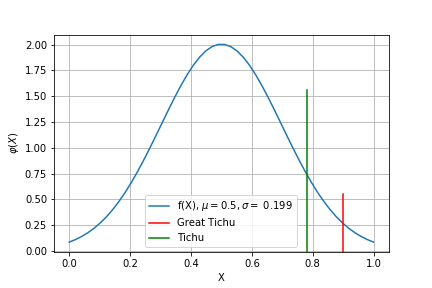
\includegraphics[width=0.5\textwidth]{Bilder/cards_distribution}
    \caption{cards distribution}
    \label{fig:meine-grafik}
    \centering
    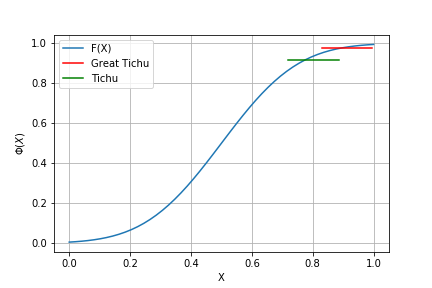
\includegraphics[width=0.5\textwidth]{Bilder/cards_distribution_cumultative}
    \caption{cards distribution cumultative}
    \label{fig:meine-grafik}
\end{figure}
\\ \\We will always use this approximation and will not discuss it furthermore.
\subsection{Subgame B.1}
To approximate the game, we will start with the most simple approach possible. A player can only pass one card, he has 14 cards on his hand. Therefore, if he passes all cards away, the average value will be $\frac{X}{14}$. This is not a perfect approximation, but it will work for the beginning. Later on, we can redefine this value if necessary. 

Keeping it easy, we will start looking at the exchange with an enemy. We only discovered one difference, whether the Player knows his Opponents strategy or not. But this difference is marginal and we will do not distinguish between these cases in this approach. 
Therefore, there is only one possible function towards an Opponent. We will call this function $\xi_O$ and assume it as normal distributed. We will set $\mu = 0$, because normally giving away one card does not change the value of your hand. According to our “stupid approach”, we will set $2\sigma = \frac{1}{14}$, because it is the value of an average card in most of the cases (further explanation in work). \\
\begin{figure}[h]
    \centering
    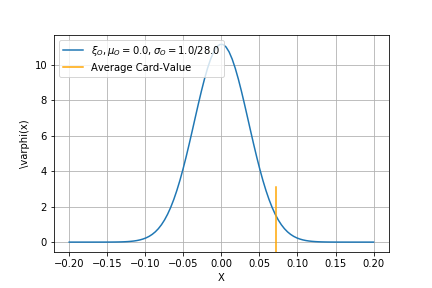
\includegraphics[width=0.5\textwidth]{Bilder/pass_function_ot}
    \caption{pass function for oppoenent player}
    \label{fig:meine-grafik}
    \centering
    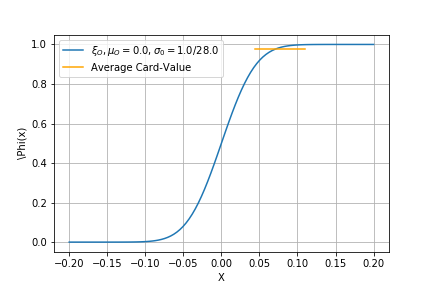
\includegraphics[width=0.5\textwidth]{Bilder/pass_function_ot_cumultative}
    \caption{pass function for the opponent player cumultative}
    \label{fig:meine-grafik}
\end{figure}
\\
The Pass-function towards your partner is more difficult to define: To realize it, let us imagine you are a new player to this game. You have no strategy and no knowledge. So every card is equal to you and as described before, the average card value is $\frac{X}{14}$. The cards are probably normal distributed within a wide range. Therefore we define $\xi_P$ as the Pass Function towards a Partner with $\mu_P = \frac{1}{14}$ and $\sigma_P = \frac{1}{14}$. 

If a player is aggressive, he will pass cards with less value and if he is defensive, he will pass cards with higher value. If he knows, his partner is defensive, he will pass lower cards and if he knows, that his partner is aggressive, he passes higher cards. This leads us to the following table:  \\
\begin{table}[h]
\caption{Table 2} \bigskip
\label{tab:my-table}
\resizebox{0.5\textwidth}{!}{%
\begin{tabular}{|l|ll|l|ll|}
\hline
\multicolumn{3}{|l|}{$\beta = 0$} & \multicolumn{3}{l|}{$\beta=1$} \\ \hline
\textit{$P_R \backslash P_P$}      & A       & D      & $P_R \backslash P_P$         & A        & D        \\ \hline
A              & -1      & +1     & A        & 0        & +2       \\
D              & -1      & +1     & D        & -2       & 0        \\ \hline
\end{tabular}%
}
\end{table}
We can construct a formula using this table: 
\begin{equation*}
z_{ji} = (1 - 2\cdot\alpha_i) + \beta_i \cdot (2\cdot\alpha_j - 1)
\end{equation*}
We will set $\mu = \mu_P + \frac{\sigma_P}{2} \cdot z_{ji}(\alpha, \beta)$. This will give us one function for $\xi_P$:
\begin{figure}[h]
    \centering
    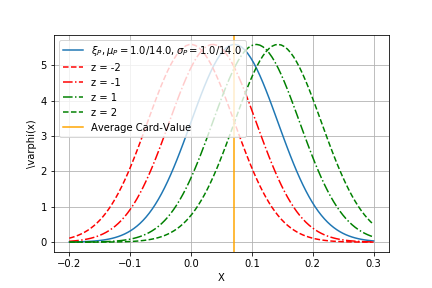
\includegraphics[width=0.5\textwidth]{Bilder/pass_function_p}
    \caption{pass function for your team partner}
    \label{fig:meine-grafik}
    \centering
    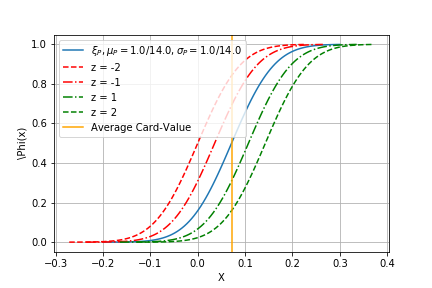
\includegraphics[width=0.5\textwidth]{Bilder/pass_function_p_cumultative}
    \caption{pass function for your teampartner cumultative}
    \label{fig:meine-grafik}
\end{figure}
\\
A card which has a negative value to player $P_i$ can have a positive value to $P_j$ (can complete a bomb). Therefore the value can change during the exchange from $\hat{\xi}_{ij}$ to $\hat{\eta}_{ij}$. In this approach, we will set $\eta_{ij} = id$, because the effect is very small in a large number of games. 

We now have created Pass-functions $\xi_{ji}$ and a Receive-Function $\eta_{ji} = 1$. We can use this functions to analyse the outcome of the Exchange-Stage $\lambda_{ji} = \xi_{ji}$. We can write $\Lambda$ using the average:
\begin{gather*}
\Lambda = \begin{pmatrix} 
1 - \xi_{21} & \xi_{12} & 0 & 0 \\
\xi_{21} & 1 - \xi_{12} & 0 & 0 \\
0 & 0 & 1 -  \xi_{43} & \xi_{34} \\
0 & 0 &  \xi_{43} & 1 - \xi_{34} \\
\end{pmatrix}
\end{gather*}

\subsection{Subgame B.2}
With the actual Tichus play there are several combinations and possibilities how this can run off. Especially decisive can be for example, who starts. Because of the combination of the cards it could be that all 4 players have the possibility to announce the Tichu. To approximate this problem as best as possible, we have considered that we simply look at the probability of winning Tichu, rather than the individual hand cards.

So first we will calculate the probability that a certain team will announce a Tichu. However, this will be done independently of the cards, because we assume that we simulate so many games that the average probabilities of winning the tichu fit better than imaginary probabilities of each card.
We assume that the team announces a tichu and not the single player. There are in theory game situations in which both team partners announce a tichu, but since we assume common knowledge, these situations are extremely rare. For example, player 1 from team 1 and player 2 from team 2 has announced a tichu. Player 3 from team 1 notices that player 1 probably won't make it and says tichu himself and wins it. This case occurs very rarely, because it requires, among other things, that player 3 has not yet played a card and is already sure that he will make the tichu and his partner will not.
In addition, we say that if both teams announce, one of the two teams will surely win the Tichu. Of course, in theory a third player could win the game (even without announcing Tichu), but this player would also have to be sure that his partner will not make it, because otherwise the common knowledge would be violated. But since this situation of absolute certainty about the cards of the partner is very rare, we neglect this case here.

So to calculate the probabilities for the announcement of the Tichu, we need 2 basic factors:
\begin{enumerate}
\item Basic aggressiveness of the players (team$_{\alpha_1}$,team$_{\alpha_2}$)
\item  Additional risk tolerance depending on the score
\end{enumerate}
The basic aggressiveness of the players is converted to a basic aggressiveness of the team. This basic aggressiveness is derived from the player model.
The willingness to take risks increases. However, this cannot be directly dependent on the player model, because due to the common knowledge, both the defensive and the aggressive player must be prepared to take extreme risks at some point.
To determine this, we have conducted a survey. It asks for the willingness to take risks in 3 categories:
\begin{enumerate}[(1)]
\item diffrence in scores
\item edge of wedge
\item own distance to victory
\end{enumerate}
The scale here was the willingness to take risks from 1 to 10, whereby in category (1) and (2) 10 meant a lot of risk and 1 normal. For (3), 1 was normal risk and 10 was particularly low risk.
 As the survey revealed, Category (1) > Category (2) > Category (3) is in the ranking. The fluctuations in category (1) are 5 points.
 For category (2) 2.5 points and in (3) 0.5 points. In this weighting, these categories are also considered in the function.
The survey revealed the following data points (based on this point we generated with numpy a regression):
\paragraph{Cat.1}
$X=[0,100,200,300,400,500,600,700,800,900]$ \\ \\
$Y=[\frac{86}{21},\frac{83}{21},\frac{96}{21},\frac{114}{21},\frac{122}{21},\frac{142}{21},\frac{150}{21},\frac{170}{21},\frac{180}{21},\frac{183}{21}]$\\
\paragraph{Cat.2}\par
$X=[100,200,300,400,500,600,700,800]$ \\ \\
$Y=[\frac{140}{21},\frac{133}{21},\frac{111}{21},\frac{105}{21},\frac{100}{21},\frac{89}{21},\frac{88}{21},\frac{93}{21}]$\\
\paragraph{Cat.3}\par
$X=[100,200,300,400,500,600,700,800]$\\ \\
$Y=[\frac{94}{21},\frac{104}{21},\frac{105}{21},\frac{92}{21},\frac{105}{21},\frac{104}{21},\frac{92}{21},\frac{94}{21}]$
\begin{figure}[h]
    \centering
    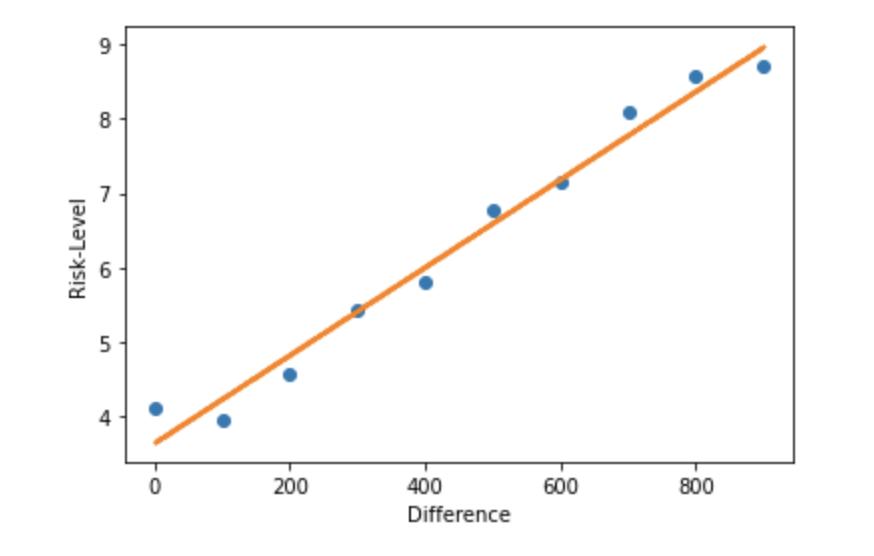
\includegraphics[width=0.5\textwidth]{Bilder/risk_level_diffrence_200steps}
    \caption{$f_1(x)=0.00591631\cdot x+3.65194805$}
    \label{fig:meine-grafik}
\end{figure}
\begin{figure}[h]
    \centering
    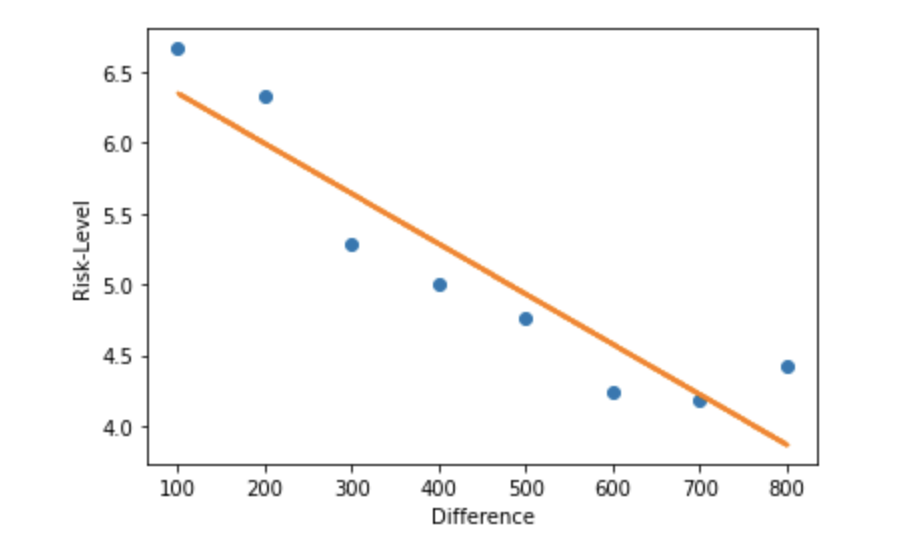
\includegraphics[width=0.5\textwidth]{Bilder/risk_level_diffrence_100steps}
    \caption{$f_2(x)=-0.00354308390\cdot x+6.70748299$}
    \label{fig:meine-grafik}
\end{figure}
\begin{figure}[h]
    \centering
    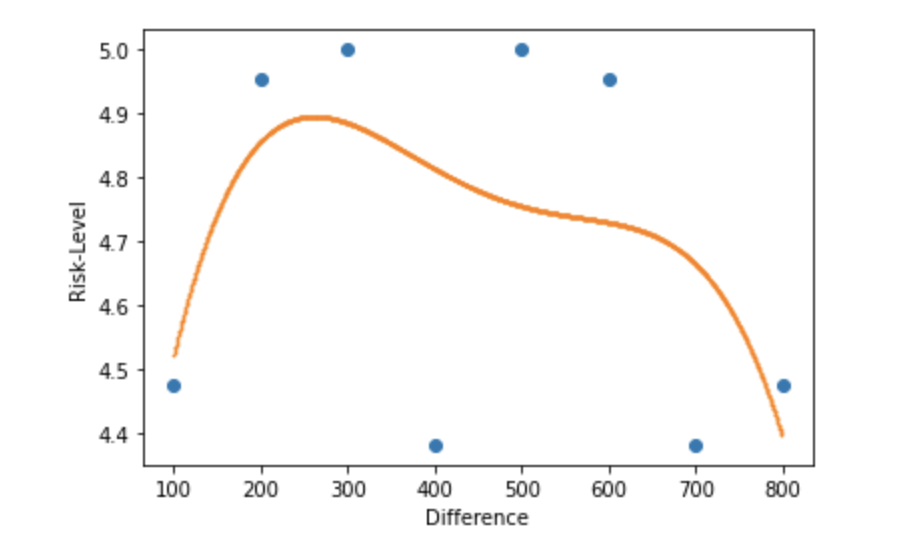
\includegraphics[width=0.5\textwidth]{Bilder/risk_level_diffrence_nonlinear}
    \caption{$f_3(x)=-3.87806638\cdot 10^{-11}\cdot x^4+7.31721982\cdot 10^{-8}\cdot x^3+ -4.95400433\cdot 10^{-5} \cdot x^2+ 1.36745860 \cdot 10^{-2} \cdot x+3.57993197$}
    \label{fig:meine-grafik}
\end{figure}
This increase should now be offset against the basic aggressiveness.
The following additional conditions are set:
If in category 1 the willingness to take risks is 8.5, the team should announce a 100$\%$ Tichu. With 4 it should have no effect.  In between it runs linear, as the function shows.
While category 1 can make a difference of up to 100$\%$, category 2 should have a maximum of 50$\%$. Again, linear.
Category 3 should bring in a maximum of 10$\%$. This function has level 4.
\begin{lstlisting}
f(play_1,play_2,t1,t2) :
    a=(play_1+play_2)/2
    if t2>=t1:
        d=(f1(t2-t1)-f1(0))/f1(900)
    else: 
        d=0
    if d>=1:
        return 1
    if t2<=200:
        b=0
    else:
        b=0.5*(f2(1000-t2)-f2(800))/
        (f2(100)-f2(800))
    if t1>=100 and t1<=800:
        c=0.1*(f3(1000-t1)-f3(800))/
        (f3(800)-f3(250))
    else:
        c=0
    if a+b-c+d>=1:
        return 1
    elif a+b-c+d>=0:
        return a+b-c+d
    else: return 0
\end{lstlisting}


In addition, there are other probabilities that must be known for the simulation. For example, the probability that a team will win the double or not. Also the probability that a player will win a Tichu must of course depend on the announcement frequency. 
Since this data should not come from somewhere, we built a web scraper and downloaded data of 13000 players from the site onlinetichu.com. From this data we have set up a function S, which assigns a probability to a player depending on his aggressiveness, with which he will win the Tichu.
So a graph of the tichu rate in relation to tichu announcements / rounds plots.
\begin{figure}[h]
    \centering
    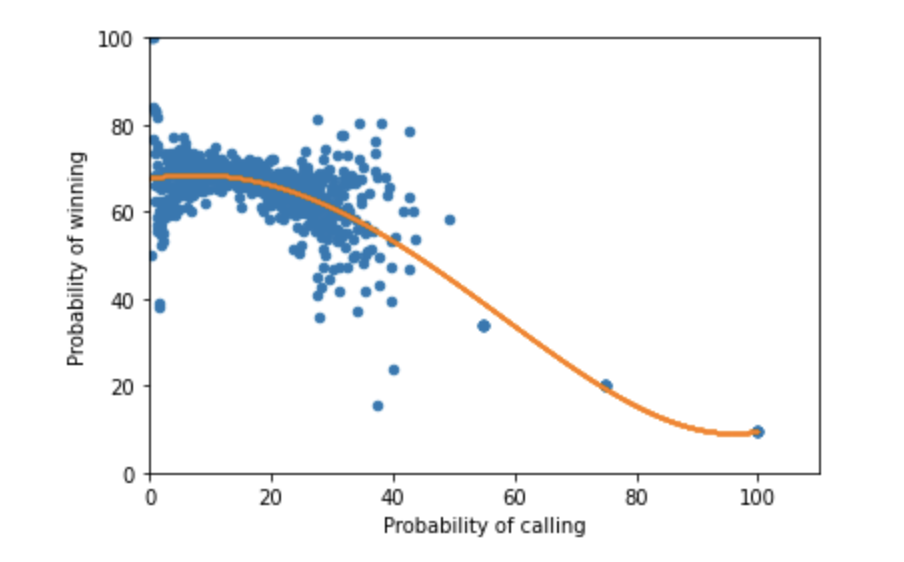
\includegraphics[width=0.5\textwidth]{Bilder/calling_winning_graph}
    \caption{$f4(x)=5.21140286\cdot 10^{-10}\cdot x^5+  7.51385614\cdot 10^{-07}\cdot x^4+  1.69471455\cdot 10^{-06}\cdot x^3+ -1.64932045\cdot 10^{-02}\cdot x^2+2.48230296\cdot 10^{-01}\cdot x + 67.7185027$}
    \label{fig:meine-grafik}
\end{figure}
The average probability for the double victory is calculated from the average of all players. So total number of doubles / total number of rounds.
\section{Simulation}
\section{Conclusion}



\end{document}

